\section{Experimental Procedure}
\label{sec:procedure}

Salicylic acid (\SI{2.002}{\gram}, \SI{14.49}{\milli\mole}) was weighed into a
dry \SI{125}{\milli\litre} Erlenmeyer flask. Acetic anhydride
(\SI{5.0}{\milli\litre}, \SI{53}{\milli\mole}) and five drops of concentrated
\ce{H2SO4} were added, and the mixture was heated in a water bath at
\SI{85}{\celsius} for \SI{15}{\minute}.

After cooling, \SI{20}{\milli\litre} of ice-cold water was added to hydrolyse the
excess anhydride, and the flask was cooled in ice until crystallisation was
complete. The crude solid was collected by vacuum filtration
(Figure~\ref{fig:product}), washed with cold water, and recrystallised from
ethanol/water.

\begin{figure}[H]
  \centering
  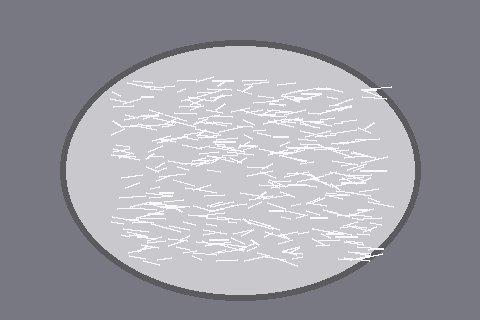
\includegraphics[width=0.55\textwidth]{product-photo.jpg}
  \caption{Recrystallised acetylsalicylic acid on the Büchner funnel.}
  \label{fig:product}
\end{figure}
